%
% numerik.tex
%
% (c) 2018 Prof Dr Andreas Müller, Hochschule Rapperswil
%
\section{Numerische Lösung gewöhnlicher Differentialgleichungen\label{section:numerik}}
\rhead{Numerische Lösungen}
In den meisten Fällen kann man gewöhnliche Differentialgleichungen
nicht in geschlossener Form lösen und ist daher gezwungen, auf ein
numerisches Lösungsverfahren zurückzugreifen.
In diesem Abschnitt sollen daher ein paar Ideen dargestellt werden,
wie man mit dem Computer angenäherte Lösungen finden kann.

%
% euler.tex -- Euler Verfahren
%
% (c) 2018 Prof Dr Andreas Müller, Hochschule Rapperswil
%
\subsection{Das Euler-Verfahren\label{subsection:euler}}
Es ist also eine autonome Differentialgleichung der Form
\[
\frac{dx}{dt} = f(x),\qquad x\in\mathbb R^n
\]
mit der Anfangsbedingung $x(0)=x_0$ numerisch zu lösen.
Die Ableitung ist definiert als der Grenzwert des Differenzenquotienten
\[
\frac{dx(t)}{dt}
=
\lim_{\Delta t\to 0}
\frac{x(t+\Delta t)-x(t)}{\Delta t}.
\]
Für genügend kleines $\Delta t$ ist der Differenzenquotient eine
(hoffentlich) ausreichend genaue Approximation für die Ableitung,
also
\begin{equation}
\frac{x(t+\Delta t)-x(t)}{\Delta t} = f(x(t))
\qquad\Rightarrow\qquad
x(t+\Delta t) = x(t) + f(x(t))\cdot \Delta t.
\label{skript:euler:differenzenquotient}
\end{equation}
Diese Formel erlaubt, die Werte $x(t)$ zu berechnen für diejenigen
Zeitpunkte $t$, die Vielfache von $\Delta t$ sind.
Schreibt man $x_k = x(k\cdot \Delta t)$, dann gilt
\begin{align*}
x(0) &= x_0\\
x_k &= x_{k-1} + \Delta t \cdot f(x_{k-1}).
\end{align*}
Dieses Verfahren heisst das {\em Euler-Verfahren}.
\index{Euler-Verfahren}%

\subsubsection{Beispiel: $y'=-ay$}
Die lineare Differentialgleichung $y'=-ay$ mit der Anfangsbedingung 
$y(0)=y_0 > 0$ kann mit dem Euler-Verfahren mit Schritten der Länge $\Delta x=h$
wie folgt gelöst werden:
\begin{align*}
y(0)&=y_0\\
y_1&=y(h) = y_0 + h\cdot y'(0) = y_0  -ah y(0) = y_0(1 - ah)
\\
y_2&=y(2h) = y_1 + h\cdot y'(h) = y_1  -ah y_1 = y_1(1-ah)
\\
&\;\;\vdots
\\
y_k&= (1-ah)^k y_0.
\end{align*}
Um den Funktionswert $x=Nh$ zu errechnen, müssen also $N$ Schritte der
Länge $h=x/N$ durchgeführt werden, oder
\[
y(x) = y_0(1-ah)^N =
y_0
\biggl(
1-\frac{ax}{N}
\biggr)^N.
\]
Erhöht man die Zahl der Schritte, erwartet man, dass das Resultat genauer
wird.
Tatsächlich ist der Grenzwert für $N\to\infty$
\[
\lim_{N\to\infty} y_0\biggl(1-\frac{ax}{N}\biggr)^N
=
y_0
e^{-ax},
\]
was natürlich die bekannte exakte Lösung der Differentialgleichung ist.
Das Eulerverfahren reproduziert also für genügend kleine Schritte 
die exakte Lösung der Differentialgleichung beliebig genau.

Das Beispiel zeigt aber auch, dass für zu grosse Schrittweite das
Verfahren unsinnige Resultate liefert.
Wenn nämlich $ah>1$ ist, dann folgt, dass
$y_k=(1-ah)^k y_0  <0$ für ungerade $k$ und $y_k < 0$ für gerade $k$.
Die numersiche Lösung liefert also negative und positive Werte,
während die exakte Lösung $y_0e^{-ax}$ nie negativ wird.

\subsubsection{Genauigkeit}
Die Genauigkeit des Euler-Verfahrens ist ziemlich beschränkt.
Um $x(1)$ in $N$ Schritten zu berechnen, muss man Zeitschritte der
Länge $\Delta t=1/N$ verwenden.
Die Approximation \eqref{skript:euler:differenzenquotient} kann mit
Hilfe der Taylor-Reihe noch etwas verbessert werden, es gilt
\begin{align}
x(t+\Delta t)
&=
x(t) + \frac{d x(t) }{dt}\cdot \Delta t
+ \frac{1}{2!}\frac{d^2x(t)}{dt^2}\cdot \Delta t^2
+ \frac{1}{3!}\frac{d^3x(t)}{dt^3}\cdot \Delta t^3
+\dots
\label{skript:euler:taylor}
\\
&=
x(t) + \frac{d x(t) }{dt}\cdot \Delta t
+ O(1/N^2).
\notag
\end{align}
Der Fehler in jedem Einzelschritt ist also von der Grössenordnung $1/N^2$.
Nach $N$ Schritten verbleibt ein Fehler in der Grössenordnung von $1/N$,
\[
x_N = x(1) + O(1/N).
\]
Um eine zusätzliche Stelle Genauigkeit zu erzielen, um den Fehler um
den Faktor 10 zu reduzieren, muss die Zahl der Schritte also zehnmal 
grösser werden.
Der Rechenaufwand für eine Steigerung der Genauigkeit um den Faktor
$s$ steigt also um den Faktor $1/s$, man sagt, das Euler-Verfahren ist
ein lineares Verfahren.

\subsubsection{Verfahren höherer Ordnung}
Die Genauigkeit des Euler-Verfahrens könnte dadurch gesteigert
werden, dass man nicht nur den ersten Term in der
Entwicklung~\eqref{skript:euler:taylor} verwendet, sondern auch
noch höhere Ableitungen berücksichtig.
Zum Beispiel könnte man die zweite Ableitung verwenden.
Diese lässt sich mit der Differentialgleichung und mit Hilfe der Kettenregel
aus
\[
\frac{d^2x}{dt^2}
=
\frac{d}{dt} \frac{dx(t)}{dt}
=
\frac{d}{dt} f(x(t))
=
Df(x(t))\cdot \frac{dx(t)}{dt}
=
Df(x(t))\cdot f(x(t))
\]
berechnen.
Allerdings ist es meistens ziemlich aufwendig, die Ableitung $Df$ von $f$ zu
berechnen.

Wir untersuchen den Genauigkeitsgewinn an Hand des Beispiels $y'=-ay$.
Die Funktion $f(y) = -ay$ hat als Ableitung die Konstante $-a$ und
die zweite Ableitung von $y$ ist
\[
y''(x) = \frac{d}{dx} y'(x) = \frac{d}{dx} (-ay(x)) = -ay'(x)=a^2 y(x)
\]
Die Taylor-Entwicklung \eqref{skript:euler:taylor} für die Schrittweite
$h=\Delta x$ wird daher
\begin{align}
y(x+h)
&=
y(x) + y'(x)h + \frac12y''(x)h^2
\notag
\\
&= y(x) - ay(x)\Delta t + \frac12 a^2 y(x)
\notag
\\
&= y(x)\cdot \biggl(1-ah+\frac12 a^2h^2\biggr)
\notag
\\
\Rightarrow\qquad\qquad
y_k&=y_0\biggl(1-ah+\frac12 a^2h^2\biggr)^k
\label{skript:euler:beschleunigt}
\end{align}
Wir erwarten, dass dieses Verfahren deutlich genauere Resultate liefert.
Die Fehler dürften von der Grössenordnung $1/N^2$ sein.
Man nennt dies ein {\em quadratisches} Verfahren.

\begin{table}
\setlength{\tabcolsep}{5pt}
\centering
\begin{tabular}{>{$}c<{$}>{$}c<{$}|>{$}c<{$}>{$}c<{$}>{$}c<{$}|>{$}c<{$}>{$}c<{$}>{$}c<{$}}
x&e^{-x}&\multicolumn{3}{c|}{Euler-Verfahren}&\multicolumn{3}{c}{beschleunigtes Verfahren \eqref{skript:euler:beschleunigt}}\\
&&h=0.1&h=0.01&h=0.001&h=0.1&h=0.01&h=0.001\\
\hline
0.0&1.00000000&1.000000&1.000000&1.000000&1.00000000&1.00000000&1.00000000\\
0.1&0.90483741&0.\underline{90}0000&0.\underline{90}4382&0.\underline{904}792&0.\underline{90}500000&0.\underline{90483}893&0.\underline{9048374}3\\
0.2&0.81873075&0.\underline{81}0000&0.\underline{81}7906&0.\underline{818}648&0.\underline{81}902500&0.\underline{81873}350&0.\underline{8187307}8\\
0.3&0.74081822&0.\underline{7}29000&0.\underline{7}39700&0.\underline{740}707&0.\underline{74}121762&0.\underline{7408}2195&0.\underline{7408182}5\\
0.4&0.67032004&0.\underline{6}56100&0.\underline{6}68971&0.\underline{670}185&0.\underline{670}80195&0.\underline{6703}2454&0.\underline{6703200}9\\
0.5&0.60653065&0.\underline{5}90490&0.\underline{60}5006&0.\underline{606}378&0.\underline{60}707576&0.\underline{60653}575&0.\underline{606530}71\\
0.6&0.54881163&0.\underline{5}31441&0.\underline{54}7156&0.\underline{548}646&0.\underline{54}940356&0.\underline{54881}716&0.\underline{5488116}9\\
0.7&0.49658530&0.\underline{4}78296&0.\underline{49}4838&0.\underline{496}411&0.\underline{49}721022&0.\underline{4965}9114&0.\underline{4965853}6\\
0.8&0.44932896&0.\underline{4}30467&0.\underline{44}7523&0.\underline{449}149&0.\underline{449}97525&0.\underline{4493}3500&0.\underline{449329}02\\
0.9&0.40656965&            0.387420&0.\underline{40}4731&0.\underline{406}386&0.\underline{40}722760&0.\underline{4065}7580&0.\underline{406569}72\\
1.0&0.36787944&0.\underline{3}48678&0.\underline{36}6032&0.\underline{367}695&0.\underline{36}854098&0.\underline{3678}8561&0.\underline{367879}50\\
\hline
\end{tabular}
\caption{Numerische Lösungen der Differentialgleichung $y'=-y$
mit dem Eulerverfahren und dem beschleunigten Verfahren 
\eqref{skript:euler:beschleunigt}.
Der Fehler im Eulerverfahren ist von der gleichen Grössenordnung wie $h$,
während er im beschleunigten Verfahren von der Grössenordnung von $h^2$ ist.
Korrekte Stellen unterstrichen.
\label{skript:euler:numerik}}
\end{table}
In Tabelle~\ref{skript:euler:numerik} sind die Resultate der numerischen
Rechnung mit beiden Verfahren mit verschiedenen Schrittweiten $h$
zusammengestellt.
Es sind nur die Werte von $y(x)$ für ganzzahlige Vielfache von $0.1$
für $x$ gelistet.
Die korrekten Stellen sind jeweils unterstrichen und bestätigen, dass
beim Euler-Verfahren der Fehler von der Grössenordnung $h$, während
er beim beschleunigten Verfahren von der Grössenordnung $h^2$ ist.

Leider ist die praktische Durchführung dieses Verfahrens erschwert durch
die Notwendigkeit der Berechnung der Matrix $Df(x)$.
Es sind jedoch Verfahren gefunden worden, mit denen die Fehlerordnung
vergrössert werden kann, ohne dass es notwendig wird, die Ableitungen
von $f$ zu berechnen.
Das wohl bekannteste solche Verfahren ist das {\em Runge-Kutta-Verfahren},
welches von vierter Ordnung ist.
Es wird im Detail vorgeführt in \cite{skript:mathsem-dgl}.




%
% octave.tex -- Differentialgleichungen mit Octave lösen
%
% (c) 2018 Prof Dr Andreas Müller, Hochschule Rapperswil
%
\subsection{Differentialgleichungen mit dem Computer lösen\label{section:octave}}
Im Abschnitt~\ref{subsection:euler} wurde das Euler-Verfahren
vorgestellt und seine Fehlerordnung untersucht.
Es wurde darauf hingewiesen, dass die lineare Fehlerordnung das Verfahren
für praktische Zwecke ungeeignet macht, da der Rechenaufwand für jede
zusätzliche Stelle Genauigkeit um einen Faktor 10 steigt.
In Computer-Programmen zur Lösung numerischer Probleme findet man daher
meistens nur Verfahren mit höherer Fehlerordnung wie zum Beispiel
das Verfahren von Runge-Kutta.

In {\em Octave} stellt die Funktion \texttt{lsode} die notwendige
\index{Octave}%
\index{lsode@\texttt{lsode}}
Funktionalität auf eine Art zur Verfügung, bei der sich der
Benutzer kaum Gedanken über die im Hintergrund verwendeten
numerischen Techniken machen muss.
Tatsächlich verwendet \texttt{lsode} ein Mehrschrittverfahren, welches
Funktionswerte an verschiedenen Stellen verwendet, um den nächsten
Funktionswert zu berechnen.
Solche Verfahren werden ebenfalls in \cite{skript:mathsem-dgl} beschrieben.

\begin{table}
\centering
\begin{tabular}{ >{$}c<{$} >{$}c<{$} >{$}c<{$} >{$}c<{$} >{$}c<{$} }
x&e^{-x}&\text{Euler}&\text{beschleunigt}&\texttt{lsode}\\
\hline
0.0&1.0000000000&1.000000&1.00000000&1.0000000000\\
0.1&0.9048374180&0.\underline{904}792&0.\underline{9048374}3& 0.\underline{90483741}56\\
0.2&0.8187307530&0.\underline{818}648&0.\underline{8187307}8& 0.\underline{8187307}365\\
0.3&0.7408182206&0.\underline{740}707&0.\underline{7408182}5& 0.\underline{740818}1957\\
0.4&0.6703200460&0.\underline{670}185&0.\underline{6703200}9& 0.\underline{6703}199847\\
0.5&0.6065306597&0.\underline{606}378&0.\underline{606530}71& 0.\underline{6065306}196\\
0.6&0.5488116360&0.\underline{548}646&0.\underline{5488116}9& 0.\underline{5488116}160\\
0.7&0.4965853037&0.\underline{496}411&0.\underline{4965853}6& 0.\underline{496585}2810\\
0.8&0.4493289641&0.\underline{449}149&0.\underline{449329}02& 0.\underline{4493289}524\\
0.9&0.4065696597&0.\underline{406}386&0.\underline{406569}72& 0.\underline{40656965}50\\
1.0&0.3678794411&0.\underline{367}695&0.\underline{367879}50& 0.\underline{36787944}04\\
\hline
\end{tabular}
\caption{Vergleich der numerische Lösung der Beispieldifferentialgleichung 
gefunden mit verschiedenen Verfahren.
Die Spalten ``Euler'' und ``beschleunigt'' enthalten die mit 
Euler-Verfahren bzw.~mit dem beschleunigten Verfahren für $h=0.001$
gefundenen Werte.
In der letzten Spalte die Resultate, die mit der Octave-Funktion 
\texttt{lsode} gefunden wurden.
\label{skript:numerik:lsode}}
\end{table}
Zur Illustration soll hier nur gezeigt werden, wie man mit \texttt{lsode}
die Beispieldifferentialgleichung lösen kann.
Dazu braucht man zunächst eine Implementation $f(x,t)$ der
Differentialgleichung.
Im Beispiel ist dies die Funktion $f(y,x)=-y$, die wir als
\lstinputlisting[style=Matlab]{chapters/3/eulerbeispiel.m}
implementieren können.
Der Funktion \texttt{lsode} müssen wir dann ausserdem noch die
Anfangsbedingung übergeben und die $x$-Werte
übergeben, für die wir Funktionswerte erhalten wollen.
Der Code
\lstinputlisting[style=Matlab]{chapters/3/eulerloesung.m}
leistet dies.
Man beachte, dass wir nirgends angeben müssen, mit welcher
Schrittweite gerechnet werden soll.
\texttt{lsode} wählt geeignete Schritte, um eine voreingestellte
Genauigkeit von 6--8 Stellen zu erreichen.
Die gewünschte Genauigkeit kann über Optionen zur Funktion
\texttt{lsode} modifiziert werden, wir verweisen in diesem Zusammenhang
auf die {\em Octave}-Dokumentation.

Die Resultate der Berechnung sind in Tabelle~\ref{skript:numerik:lsode}
zusammengstellt.
Man beachte, dass am Ende des Intervalls eine Genauigkeit von
8 Stellen erreicht wird, besser als mit dem beschleunigten
Verfahren.
Nicht aus der Tabelle ersichtlich ist die Anzahl der Aufrufe der
Funktion \texttt{f}.
Für das Eulerverfahren und das beschleunigte Verfahren sind bei
der Schrittweite $h=0.001$ genau 1000 Aufrufe notwendig.
Die Funktion \texttt{lsode} ruft dagegen die Funktion \texttt{f}
nur 49 mal auf.
Da die Auswertung der Funktion \texttt{f} in der Praxis meistens
der dominierende rechnerische Aufwand ist, ist \texttt{lsode}
den anderen beiden Verfahren auf gerade zu spektakuläre Weise überlegen.









%
% elemente.tex -- 
%
% (c) 2018 Prof Dr Andreas Müller, Hochschule Rapperwil
%
\subsection{Lineare Differentialgleichungen\label{subsection:lindgl}}
Für eine lineare Differentialgleichung ist die Funktion $f(x)$ linear
in $x$.
Sind $x_1(t)$ und $x_2(t)$ Lösungen der Differentialgleichung
für Anfangswerte $x_1(0)$ und $x_2(0)$, dann ist
$x_1(t)+x_2(t)$ eine Lösung der Differentialgleichung für die
Anfangsbedingung $x_1(0)+x_2(0)$.

\begin{figure}
\centering
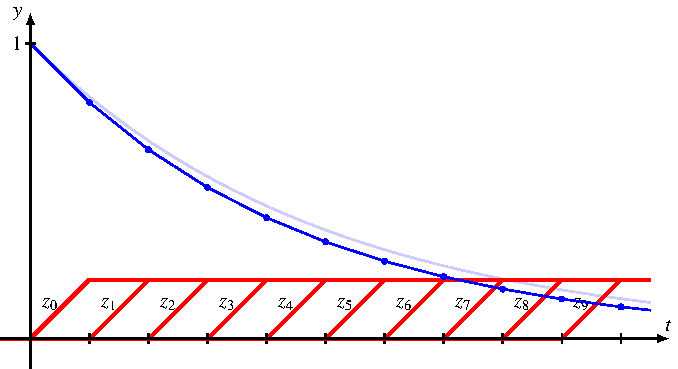
\includegraphics{chapters/3/slopes.pdf}
\caption{Basisfunktionen, aus denen die interpolierte Lösung $\tilde{x}(t)$
durch Linearkombination gefunden werden kann.
\label{skript:elemente:slopes}}
\end{figure}

Die Linearität ermöglicht also, Lösungen der Differentialgleichung
als Linearkombination von Lösungen zu finden.
Das Euler-Verfahren hat diskrete Werte $x_k=x(hk)$ gefunden,
die Werte $x(t)$ für $t$ zwischen den Punkten $t_k=hk$ können
durch Interpolation gefunden werden, wir nennen diese interpolierte
Funktion $\tilde{x}(t)$.
Für einen Punkt $t$ zwischen $t_k$ und $t_{k+1}$ ist dann
\[
\tilde{x}(t) = x(t_k) + (t-t_k)\cdot f(x_k, t_k).
\]
Dies kann man auch als Linearkombination von Funktionen
schreiben.
Wir betrachten die Funktionen
\[
z_k(t)
=
\begin{cases}
0&\qquad t < t_k\\
t-t_k&\qquad t_k \le t < t_{k+1}\\
h&\qquad t_{k+1} \le t,
\end{cases}
\]
wie sie in Abbildung~\ref{skript:elemente:slopes} rot dargestellt sind.
Damit wird die interpolierte Funktion zu einer Linearkombination:
\[
\tilde{x}(t)
=
x_0 + f(x_0)\cdot z_0(t) + f(x_1)\cdot z_1(t) + f(x_2) \cdot z_2(t) + \dots
=
x_0
+
\sum_{k=0}^n f(x_k) z_k(t).
\]
Diese Lösung ist in Abbildung~\ref{skript:elemente:slopes} blau dargestellt.
Hellblau ist die exakte Lösung $y=e^{-x}$.
Die Lösung $\tilde{x}(t)$ ist also eine Linearkombination
\[
\tilde x(t) = x_0 + \sum_{k=0}^\infty a_k\cdot z_k(t)
\]
der Funktionen $z_k(t)$ schrieben können.
Wir brauchen nur eine Methode, mit der die Koeffizienten $a_k$ bestimmt
werden können.
Da die Funktionen $y_k$ linear sind, könnten wir $\tilde{x}(t)$ in die 
Differentialgleichung einsetzen:
\begin{equation}
\sum_{k=0}^\infty
a_k\frac{d\tilde{z}_k(t)}{dt}
=
f(x_0) + \sum_{k=0}^\infty z_k(t) f(a_k).
\label{skript:elemente:eingesetzt}
\end{equation}
Leider funktioniert das nicht, weil die Funktionen $z_k$ nicht differenzierbar
sind.
Sie sind aber rechtseitig differenzierbar, der Grenzwert
\[
\lim_{\Delta t \to 0+} \frac{z_k(t+\Delta t)-z_k(t)}{\Delta t}
=
\begin{cases}
0&\qquad t<t_k\\
1&\qquad t_k\le t< t_{k+1}\\
0&\qquad t_{k+1} \le t
\end{cases}
\]
existiert immer.
Wenn wir in der Gleichung also überall mit rechtsseitigen Ableitungen
arbeiten, dann bleiben in \eqref{skript:elemente:eingesetzt} an den
Punkten $t_j$ nur wenige Terme übrig.
Auf der linken Seite steht
\begin{equation}
\sum_{k=0}^\infty
a_k\frac{d\tilde{z}_k(t_j)}{dt}
=
a_j,
\label{skript:elemente:links}
\end{equation}
auf der  rechten
\begin{equation}
f(x_0) + \sum_{k=0}^\infty z_k(t_j) f(a_k)
=
f(x_0) + \sum_{k=0}^{j-1} hf(a_k)
=
f\biggl(x_0 + \sum_{k=0}^{j-1} ha_k\biggr).
\label{skript:elemente:rechts}
\end{equation}
Zusammen mit \eqref{skript:elemente:links} folgt
\[
\begin{aligned}
a_0 &= f(x_0)                 &&          &    & \\
a_1 &= f(x_0 + ha_0) = f(x_1) &&\text{mit}&x_1 &= x_0 + ha_0\\
a_2 &= f(x_1 + ha_1) = f(x_2) &&\text{mit}&x_2 &= x_1 + ha_1\\
    &\;\;\vdots
\end{aligned}
\]
Die Idee, die Funktion $x(t)$ als Linearkombination $\tilde{x}(t)$
der Funktionen zu approximieren, führt also auf natürliche Weise
auf das Euler-Verfahren.

Diese Idee lässt sich auf auch auf nichtlineare Differentialgleichungen
verallgemeinern.
Die Tatsache, dass $f(x)$ linear ist in $x$ hat die Hemmschwelle etwas
heruntergesetzt, die Lösung als Linearkombination anzusetzen.
Das Euler-Verfahren macht aber keine solche Voraussetzungen.
Das einzige, was sich ändert, wenn $f(x)$ nicht mehr linear ist,
ist dass die rechte Seite nach Einsetzen der Linearkombination
etwas komplizierter wird.

Dies motiviert ein ganz allgemeines Verfahren zur Lösung von
Diffentialgleichungen:
\begin{enumerate}
\item Wähle eine Familie von Funktionen $z_k(t)$ und setze die Lösung
als Linearkombination
\[
\tilde{x}(t) = \sum_{k=0}^\infty a_k\cdot z_k(t), \qquad a_k\in\mathbb R^n
\]
an.
\item Setze den Ansatz $\tilde{x}(t)$ in die Differentialgleichung ein
und leite daraus Gleichungen für die Koeffizienten $a_k$ ab.
\item Die Gleichungen für $a_k$ können unter Umständen sehr schwierig 
zu lösen sein.
Es kann sogar sein, dass die Gleichungen überbestimmt sind, dass die
$a_k$ also nur zum Beispiel im Sinne der kleinsten Quadrate bestimmt
werden können.
\end{enumerate}
In Abschnitt \ref{section:pdeloesungen} wird diese Idee weiterentwickelt
und gezeigt, wie sie für geeignetere Familien von Funktionen als die $z_k(t)$
erfolgreich sein kann.



